\documentclass[12pt, twoside]{article}
\usepackage[letterpaper, margin=1in, headsep=0.2in]{geometry}
\setlength{\headheight}{0.6in}
%\usepackage[english]{babel}
\usepackage[utf8]{inputenc}
\usepackage{microtype}
\usepackage{amsmath}
\usepackage{amssymb}
%\usepackage{amsfonts}
\usepackage{siunitx} %units in math. eg 20\milli\meter
\usepackage{yhmath} % for arcs, overparenth command
\usepackage{tikz} %graphics
\usetikzlibrary{quotes, angles}
\usepackage{graphicx} %consider setting \graphicspath{{images/}}
\usepackage{parskip} %no paragraph indent
\usepackage{enumitem}
\usepackage{multicol}
\usepackage{venndiagram}

\usepackage{fancyhdr}
\pagestyle{fancy}
\fancyhf{}
\renewcommand{\headrulewidth}{0pt} % disable the underline of the header
\raggedbottom
\hfuzz=2mm %suppresses overfull box warnings

\usepackage{hyperref}

\fancyhead[LE]{\thepage}
\fancyhead[RO]{\thepage \\ Name: \hspace{4cm} \,\\}
\fancyhead[LO]{BECA / Dr. Huson / Geometry\\*  Unit 12: Trigonometry \\* 20 March 2023}

\begin{document}

\subsubsection*{12.6 Trigonometric situations \hfill HSG.SRT.C.8}
\begin{enumerate}
\item Shown is a building with student $A$ on the ground waving up to student $B$. Point $A$ is 40 feet from the base of the building, and the angle of elevation from $A$ to $B$ is $37^\circ$.

Find how high up student B is from the ground to the \emph{nearest foot}. \hfill (not to scale)
  \begin{flushright}
    \begin{tikzpicture}[scale=0.3]
      %\draw [-, thick] (0,0)--(35:23);
      \draw [-, thick] (-4,0)--
      (0,0)--
        (17,0)--
        (22,0)--
        (22,10)--(17,10)--(17,0);
      \draw [fill] (0,0) circle [radius=0.1] node[above left]{$A$};
      \draw [fill] (17,10) circle [radius=0.1] node[above right]{$B$};
      \draw [dashed] (0,0)--(17,10);
      \node at (3.8, 0)[above]{$37^\circ$};
      \node at (11, 0)[above]{distance = 40 ft};
      \node at (19.5, 5)[above]{school};
    \end{tikzpicture}
    \end{flushright}

\item Yolanda is making a springboard to use for gymnastics. She has 8-inch-tall springs and wants to form a $16.5$ angle with the base, as modeled in the diagram below.
\begin{center}
  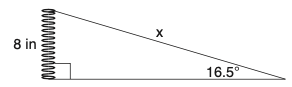
\includegraphics[scale=0.6]{../graphics/trig-spring.png}
\end{center}
To the \emph{nearest tenth of an inch}, what will be the length of the springboard, $x$? \vspace{4cm}

\item A child sleds from the top of a hill to a group of friends standing at the base of the hill. The hill is 20 feet tall, and the distance from the sledder to the group of friends is 110 feet. Find the angle of the incline $x$.
\begin{flushright}
  \begin{tikzpicture}[scale=1.1]
    \draw [thick] (10,0)--(0,0)--(10,2.0)--cycle;
    \draw [thick, ->] (1.5,0) arc [start angle=0, end angle=11.3, radius=1.5];
    \node at (1,0)[below]{Incline $=x^\circ$};
    \node at (10,1.2)[left]{$20$};
    \node at (5,1.6)[below]{$110$};
  \end{tikzpicture} 
\end{flushright}\vspace{4cm}
  
\newpage
\item A pirate, who is two meters tall, is standing on a mast 8 meters tall. Looking down, the pirate sees an enemy ship 45 meters away.

  Find the angle of depression to the nearest degree.
  \begin{center}
      \begin{tikzpicture}[scale=1.1]
        \draw [thick] (10,0)--(0,0)--(10,2.0)--cycle;
        \draw [dashed, <-] (5,2)--(10,2.0);
        \draw [thick, ->] (8.5,2) arc [start angle=180, end angle=191.3, radius=1.5];
        \node at (5.5,2)[below]{Angle of depression $ =\theta^\circ$};
        \node at (10,1.2)[right]{$h=8+2$ meters};
        \node at (6,0)[below]{$45 \,\rm{meters}$};
        \node at (0,0)[below right]{Enemy ship};
      \end{tikzpicture}
    \end{center} \vspace{4cm}
    
\item A snowman is standing 6 meters away from the base of a set of monkey bars, looking up at a boy $x$ meters off the ground. The snowman is 1 meter tall and the angle of elevation of his view to the boy is $18.5^\circ$.

    Find the height of the boy off the ground.
    
      \hfill (not drawn to scale)
      \begin{flushright}
        \begin{tikzpicture}[scale=0.6]
          \draw [-, dashed] (0,2)--(3,2);
          \draw [-, thick] (-4,0)--
          (0,0)--
            (10,0)--(10,6)--(12,6);
          \draw (0,0.75) circle [radius=0.75];
          \draw (0,2) circle [radius=0.5];
          \draw [fill] (10,6) circle [radius=0.1] node[above right]{Boy};
          \draw [dashed] (0,2)--(10,6);
          \node at (3, 2)[above]{$18.5^\circ$};
          \node at (12, 2)[above]{Bars};
          \node at (12.5, 3)[above]{Monkey};
        \end{tikzpicture}
        \end{flushright}

\newpage
\item A drone flying at an altitude of 1,800 meters is observed twice. The first time the angle of elevation is $7.2^\circ$ and exactly one minute later the angle of elevation is $9.7^\circ$. \\[0.25cm]
Find the distance the drone flies over the minute and its speed in kilometers per hour.

\hfill (not drawn to scale)
\begin{flushright}
  \begin{tikzpicture}[scale=1.1]
    \draw [thick] (10,0)--(0,0)--(10,2.0)--cycle;
    \draw (10,0)++(-0.3,0)--++(0,0.3)--+(0.3,0);
    \draw [dashed] (0,0)--(7,2.0);
    \draw [dashed, <-] (6,2)--(10,2);
    \draw [thick, ->] (1.5,0) arc [start angle=0, end angle=11.3, radius=1.5];
    \draw [thick, ->] (2.5,0) arc [start angle=0, end angle=15.3, radius=2.5];
    \node at (1,0.7)[above]{Angles of elevation};
    \node at (1.5,0)[below]{$7.2^\circ$};
    \node at (3,0)[above]{$9.7^\circ$};
    \node at (10,1.2)[left]{$1800$};
    \node at (8,2)[above]{drone};
  \end{tikzpicture} 
\end{flushright}
\vspace{6cm}

\item The vertices of quadrilateral $MATH$ have coordinates $M(-4,2)$, $A(-1,-3)$, $T(9,3)$, and $H(6,8)$. \\[0.5cm]
Prove that quadrilateral $MATH$ is a parallelogram.

\end{enumerate}
\end{document}
  